\begin{figure*}[tb]
	\centering
	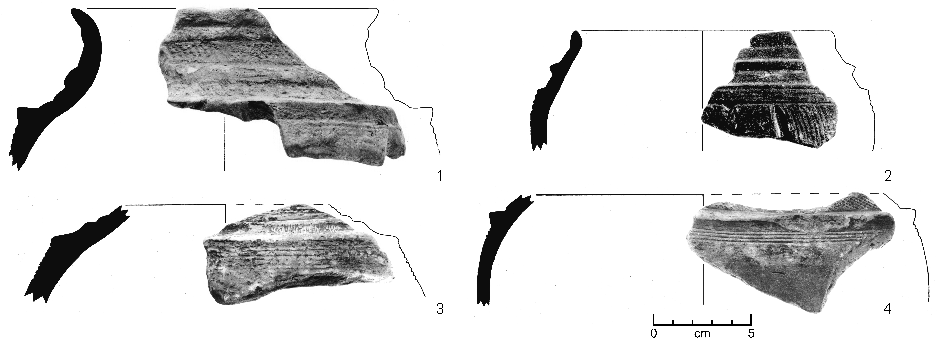
\includegraphics[width=\textwidth]{fig/BDG-Typen.pdf}
	\caption{Bondongo-Gruppe: Typvertreter aus Loka (Fpl.~193) und \mbox{Ngbanja} (Fpl.~199).\\1:~Taf.~4.1; 2:~Taf.~6.11; 3:~Taf.~3.1; 4:~Taf.~4.3.}
	\label{fig:BDG_Typverteter}
\end{figure*}

\subsubsection{Bondongo-Gruppe}\label{sec:BDG-Gr}

Vertreter des im Inneren Kongobecken weit verbreiteten Bondongo-Stils\footnote{Funde aus dem südöstlich des Lac Tumba  gelegene Ortes Bondongo-Losombo (Fpl.~1) bildeten den Ausgangspunkt für die ab den späten 1970er Jahren durchgeführten Feldarbeiten des \textit{River Reconnaissance Project} \parencites[siehe][]{Sulzmann.1960}{Eggert.1980b}.} \parencites[""128--139]{Wotzka.1995} finden sich ebenfalls im nordwestlichen Kongobecken, vornehmlich entlang des Unterlaufs des \mbox{Ubangi}, am 1987 befahrenen Abschnitt des Kongo und dem unteren \mbox{Sangha} (Abb.~\ref{fig:BDG_Verbreitung}). Die nördlichste Fundstelle von Bondongo-Keramik im Arbeitsgebiet ist \mbox{Ngbanja} am mittleren \mbox{Ubangi} (Fpl.~199). Im Süden reicht das Verbreitungsgebiet bis nach Bonga an der Mündung des \mbox{Sangha} (Fpl.~238). Obschon auch \textsc{Wotzka} (ebd. 135) auf formale wie ornamentale Ähnlichkeiten zur Imbonga-Keramik hinweist (ebd. ""59--68), spiegelt die \enquote{reichverzierte, rundbodige Keramik [der Bondongo-Gruppe] mit prononciertem Schulterabsatz} und flächiger \textit{banfwa-nfwa}-Verzierung einen deutlich jüngeren zeitlichen Abschnitt in der regionalen Sequenz wider. \textsc{Wotzka} (ebd. 224\,f.) fasst das im Zusammenhang mit der Keramik der Bondongo-Gruppe zu beobachtende zeitgleiche Bestehen regional determinierter, jedoch untereinander eng verwandter Stilgruppen zu einem \textit{Bondongoid-Horizont} zusammen, der neben der Bondongo-Gruppe auch die Stilgruppen Bekongo, Wafanya, Besongo und Wema umfasst.\footnote{Es gilt an dieser Stelle auf den Unterschied zu dem von \textcite[285--287]{Eggert.1983} verwendeten Terminus \enquote{Horizont} hinzuweisen, der der Zusammenfassung regionaler Ausprägungen ähnlicher keramischer Merkmale diente (ebd. 295). \textcite[224\,f.]{Wotzka.1995} hingegen fasst, in Anlehnung an Arbeiten von \textcites[108--116]{Kroeber.1944}[49]{Willey.1945}, zeitgleiche und miteinander in Beziehung stehende Stilgruppen zu \enquote{Stilhorizonten} zusammen. Siehe Kap.~\ref{sec:Horizonte}.} Im nordwestlichen Kongobecken ließen sich an 14 Fundplätzen (Abb.~\ref{fig:BDG_Verbreitung}) insgesamt elf GE sicher der Bondongo-Gruppe zuordnen, bei weiteren 37~GE war eine Zuweisung nur unter Vorbehalt möglich. Dies lässt sich vor allem auf den Umstand zurückführen, dass keine der GE aus einem ausgegrabenen Befundzusammenhang stammt und alle Stücke bei Oberflächensurveys gefunden wurden. Daraus ergab sich ebenfalls eine auffällig schlechte Erhaltung sowie starke Fragmentierung. Insgesamt 63~\% aller der Bondongo-Gruppe zugewiesenen GE sind kleiner als 70\,$\times$\,70\,mm. Das Inventar besteht zu großen Teilen aus Fragmenten der Gefäßwandung (74~\%), während Randstücke nur einen geringen Anteil ausmachen (25~\%). Das Gros der Stücke stammt aus Maberu am Kongo (Fpl.~235; 30~\%), \mbox{Ngbanja} am mittleren \mbox{Ubangi} (23\,\%) und Loka am unteren \mbox{Ubangi} (Fpl.~193; 13\,\%). An allen anderen Fundstellen kommen GE der Bondongo-Gruppe lediglich in sehr geringen Stückzahlen oder als Einzelfunde vor. 

\paragraph{Technologische Merkmale}\hspace{-.5em}|\hspace{.5em}%
Wie auch im Inneren Kongobecken, wo sich Bondongo-Keramik in technologischer Hinsicht lediglich durch eine vergleichsweise geringe Wandungsstärke auszeichnet (ebd. 128), dominieren auch bei den Stücken aus dem nordwestlichen Kongobecken die charakteristischen, kaum nichtplastische Partikel aufweisenden \textit{Fabrics} 1 (80\,\%) und 2 (6\,\%). In Einzelfällen weisen GE aber auch Zusätze in Form von zerstoßener Keramik -- \textit{Schamott} -- auf (Taf.~33.9). Ebenfalls in Einzelfällen lässt sich feiner Quarzsand oder ausgebrannte Organik beobachten. Mit Blick auf die Wandungsstärke der Bondongo-Gefäße zeigen sich im Arbeitsgebiet keine Auffälligkeiten. Die mittlere Dicke der Wandungen beträgt 7,8\,mm, mit einer Varianz von 4,9\,mm. Die Oberflächen der Scherben sind fast ausschließlich gut geglättet (92\,\%). Mit Blick auf die Brennfarbe der genutzten Tone ergibt sich ein deutlicher Fokus auf Färbungen, die auf die Nutzung weißbrennender Tone hinweisen (54\,\%), während Hinweise auf rotbrennende Tone nur selten beobachtet wurden (12\,\%). Die restlichen 34\,\% der Stücke lassen keine Ansprache zu. 

\begin{figure*}[p]
	\centering
	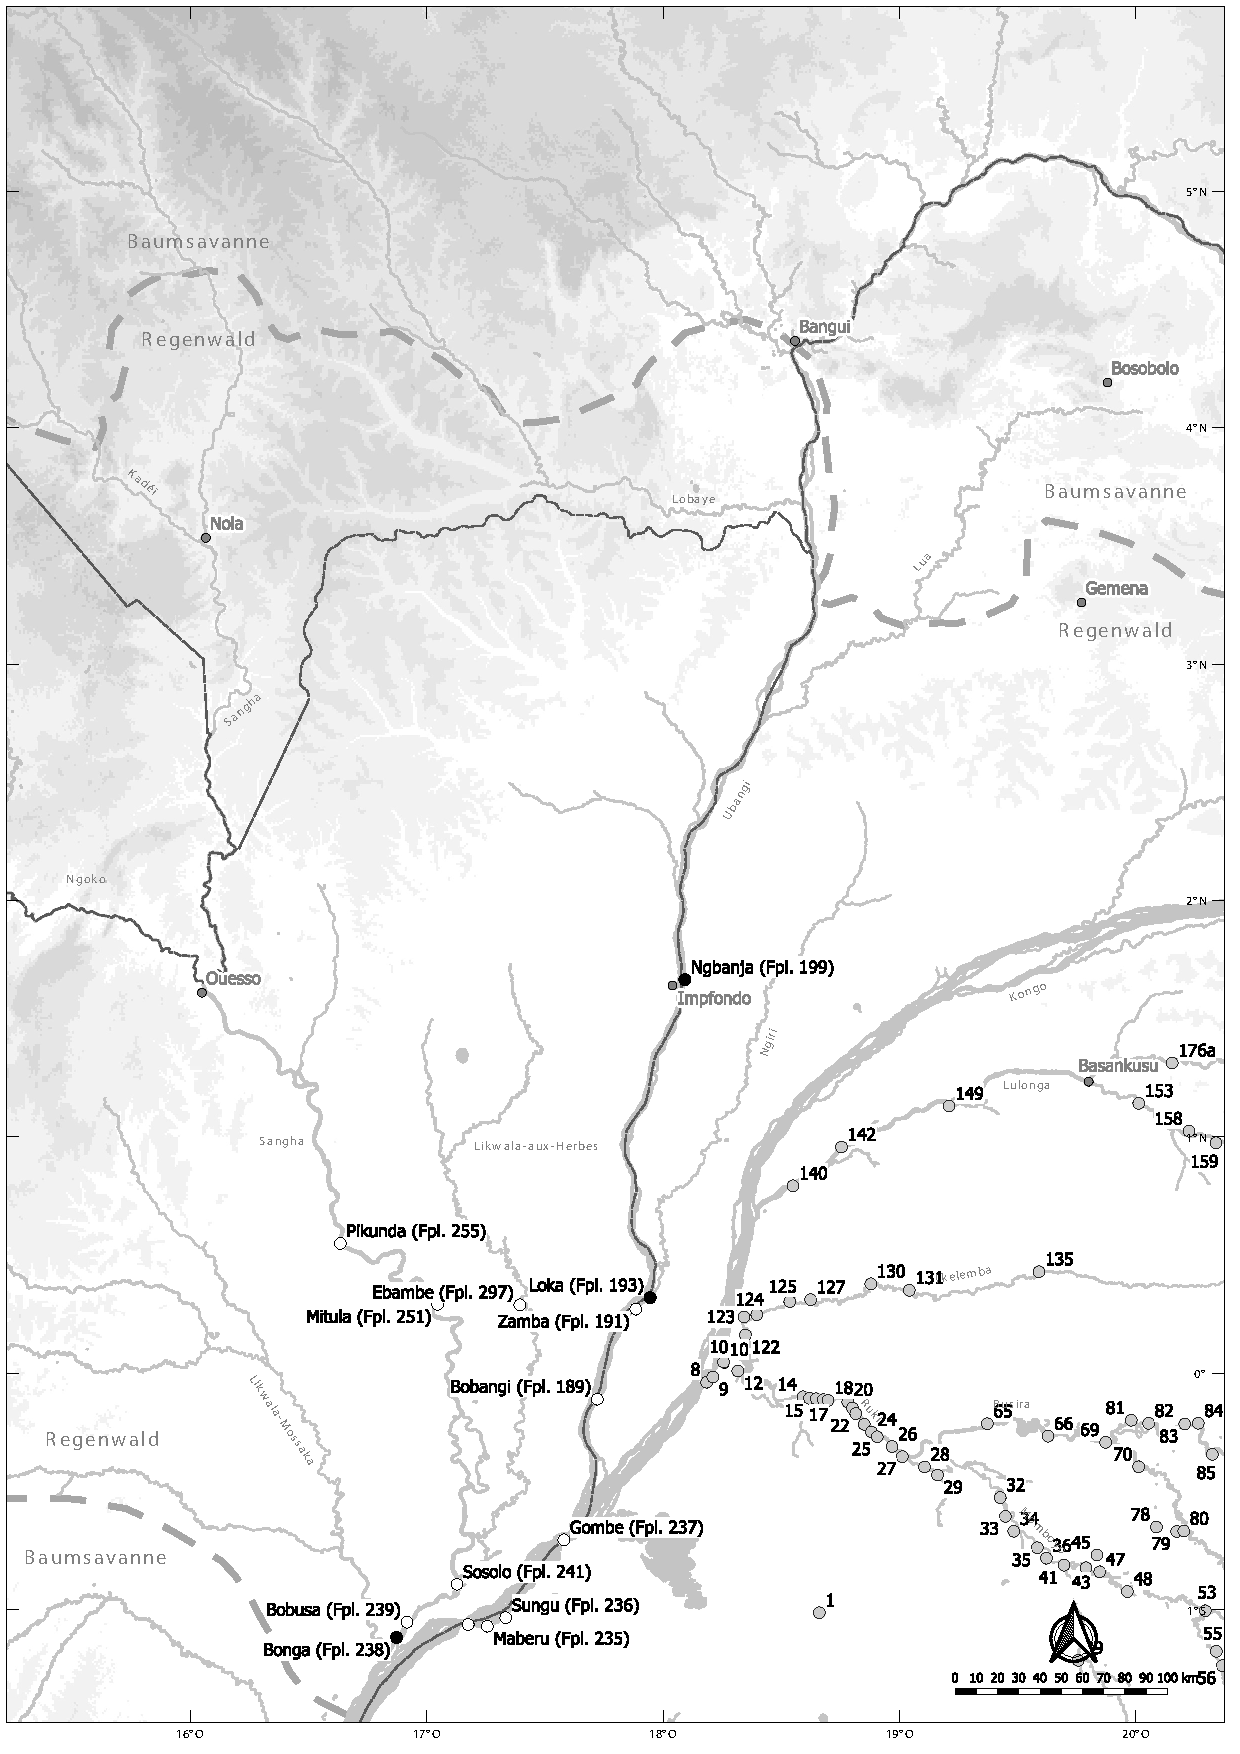
\includegraphics[width=\textwidth]{fig/BDG_Verbreitung.pdf}
	\caption{Bondongo-Gruppe: Verbreitung im Arbeitsgebiet sowie im Inneren Kongobecken \parencite[grau nach][562--563 Karte 11]{Wotzka.1995}.}
	\label{fig:BDG_Verbreitung}
\end{figure*}

\paragraph{Formen}\hspace{-.5em}|\hspace{.5em}%
Eines der kennzeichnenden Merkmale des Bondongo-Stils sind Gefäße mit geschweifter Wandung und prononcierter Gefäßschulter, die häufig spitz zulaufende plastische Leisten aufweisen (Abb.~\ref{fig:BDG_Typverteter}). Von den insgesamt 48 individuell aufgenommenen GE der Bondongo-Gruppe im nordwestlichen Kongobecken kann bei sieben die Gefäßform sicher bestimmt werden. Bei 22 weiteren GE ist eine Ansprache nur unter Vorbehalt möglich. Den größten Anteil bilden Gefäße mit geschweifter Wandung, deutlich abgesetzter Gefäßschulter und ausgeprägtem Halsbereich vom Typ C2 (76\,\%). Daneben finden sich Gefäße ohne stark abgesetzte Schulter vom Typ C1 (10\,\%) sowie mit stark konvexer Wandung und ohne ausgeprägten Halsbereich vom Typ D1 (10\,\%). Eine GE lässt sich als Gefäß mit geschweifter Wandung, ohne ausgeprägten Schulter- und Halsbereich ansprechen (Typ E1; 4\,\%).\footnote{Die geschilderten Anteile entsprechen dem von \textsc{Wotzka} (1995: 128--130) im Inneren Kongobecken beschriebenen Formenspektrum. Die zahlreichen Gefäße des Typs C2, mit geschweifter Wandung sowie ausgeprägtem Schulterabsatz und Gefäßhals entsprechen der von \textsc{Wotzka} (ebd. 128\,f.) beschriebenen Gefäßform 53, die 66\,\% aller Bondongo-Gefäße im Inneren Kongobecken beschreibt.} Bei 15 der im Arbeitsgebiet identifizierten GE der Bondongo-Gruppe kann die Form des Randes angesprochen werden. Es handelt sich fast ausschließlich um ausbiegende Formen (93\,\%), wobei gerade (B1; 40\,\%) sowie konkav ausbiegende Formen (B2; 33\,\%) deutlich überwiegen. Die Randlippen sind größtenteils rund (M1; 43\,\%) oder spitz (M2; 36\,\%) ausgearbeitet. Der häufig konkav (49\,\%) oder kegelförmig (26\,\%) ausgeführte Halsbereich geht regelhaft in eine mit einer plastischen Leiste (48\,\%) oder einem Absatz (19\,\%) versehenen Gefäßschulter über. Dezidierte Bodenstücke des Bondongo-Stils konnten nicht beobachtet werden. Die Gefäßböden der Bondongo-Keramik im Inneren Kongobecken sind zu großen Teilen (70\,\%) rund ausgearbeitet (B1; ebd. 131 Tab.~57).

\paragraph{Verzierungen}\hspace{-.5em}|\hspace{.5em}%
Die Verzierungen der Bondongo-Keramik im Arbeitsgebiet bestehen zu großen Teilen aus horizontalen Rillen (Tab.~\ref{tab:Verzierungselemente}: 02.1; 45\,\%), gefolgt von flächigem \textit{banfwa-nfwa} (Tab.~\ref{tab:Verzierungselemente}: 08; 16\,\%). Insgesamt machen Ritzungen (Tab.~\ref{tab:Verzierungselemente}: 01) und Riefen (Tab.~\ref{tab:Verzierungselemente}: 02) über 60\,\% aller beobachteten Verzierungselemente aus. Horizontale Rillen (Tab.~\ref{tab:Verzierungselemente}: 02.1) finden sich auf allen Gefäßpositionen, von der Innenseite der Ränder bis zum Bauchbereich der Gefäße. Am häufigsten lassen sie sich aber direkt unterhalb der plastischen Leiste im Schulterbereich der Gefäße beobachten (Abb.~\ref{fig:BDG_Typverteter}). Die Gefäßunterteile sowie die Innenseite im Bereich des Randes sind in der Regel mit \textit{banfwa-nfwa} verziert.\footnote{Da dieses Merkmal jedoch eine weite Verbreitung aufweist und zum Beispiel auch innerhalb der Ebambe- (Kap.~\ref{sec:EBA-Gr}) und der Botendo-Gruppe (Kap.~\ref{sec:BOT-Gr}) anzutreffen ist, kann es nur bedingt als Unterscheidungskriterium herangezogen werden.} Im Inneren Kongobecken bilden Ritztechniken sowie \textit{banfwa-nfwa} den Schwerpunkt der Ornamentik (\textsc{Wotzka} 1995: 131). Nahezu alle Gefäßbereiche sind verziert, obschon der Fokus auf der Schulterregion der Gefäße liegt. Hier fanden sich 35\,\% aller aufgenommenen Verzierungselemente.\footnote{Diese Zahlen müssen zum Teil auch auf die diagnostischen plastischen Leisten auf den Gefäßschultern zurückgeführt werden.} Grundsätzlich ist die Bondongo-Keramik eine der am reichhaltigsten verzierten Stile des Kongobeckens.


\paragraph{Datierung}\hspace{-.5em}|\hspace{.5em}%
Für die ausschließlich bei Surveys von Dorfoberflächen erschlossenen Funde der Bondongo-Gruppe im nordwestlichen Kongobecken liegen keine direkten Radiokohlenstoffdatierungen vor. \textsc{Wotzka} (ebd. 138) gibt für die Datierung der Bondongo-Keramik des Inneren Kongobeckens einen Zeitraum zwischen 1000--1400 n.~Chr. an. Von den insgesamt 14 Radiokohlenstoffdatierungen, die Kontexten mit Bondongo-Keramik im Inneren Kongobecken zuzuordnen sind, werden ausschließlich neun von \textsc{Wotzka} (ebd. 138 Tab.~58 Nr.~3--11) als repräsentativ angesehen.\footnote{Zwei aus Bolondo am Tshuapa (Fpl.~96) stammende und in Hannover datierte Proben werden von \textsc{Wotzka} (1995: 138 Tab.~58 Nr.~1--2) als zu alt angesehen, während zwei Datierungen aus Bamanya (Fpl.~12) sowie eine aus Mbandaka (Fpl.~10; ebd. 138 Tab.~58 Nr.~12--14) zu jung für die Laufzeit des Bondongo-Stils sind.}


\paragraph{Verbreitung}\hspace{-.5em}|\hspace{.5em}%
Das Verbreitungsgebiet von Bondongo-Keramik im nordwestlichen Kongobecken beschränkt sich auf den südlichsten Teil des Arbeitsgebietes, vornehmlich den Unterlauf der Flüsse \mbox{Ubangi} sowie \mbox{Sangha} und den prospektierten Abschnitt des Kongo. Funde des Bondongo-Stils sind an 14 Fundstellen belegt (Abb.~\ref{fig:BDG_Verbreitung}). Vom \mbox{Likwala}-\mbox{aux}-\mbox{Herbes} ist lediglich aus Ebambe (Fpl.~297) eine mögliche Bondongo-Scherbe belegt. Während sich an den meisten dieser Fundstellen nur vereinzelte Stücke fanden, stammt das Gros des Inventars dieser Stilgruppe aus \mbox{Ngbanja} am mittleren \mbox{Ubangi} (Fpl.~199) -- zugleich die nördlichste Fundstelle -- und Maberu (Fpl.~235) am Kongo. Keines der Stücke stammt aus einem ergrabenen Kontext, alle Scherben wurden bei Oberflächenbegehungen entdeckt.